\documentclass[10pt,executivepaper]{article}
\usepackage[utf8]{inputenc}
\usepackage[spanish]{babel}
\usepackage{amsmath}
\usepackage{amsfonts}
\usepackage{amssymb}
\usepackage{graphics}
\usepackage{graphicx}
\usepackage[left=2cm,right=2cm,top=2cm,bottom=2cm]{geometry}
\usepackage{imakeidx}
\makeindex[columns=3, title=Alphabetical Index, intoc]
\usepackage{listings}
\usepackage{xcolor}
\usepackage{multicol}
\usepackage{changepage}
\usepackage{float}
\usepackage{cite}
\usepackage{url}
\usepackage{pdflscape}
\usepackage{listingsutf8}

\definecolor{codegreen}{rgb}{0,0.6,0}
\definecolor{codegray}{rgb}{0.5,0.5,0.5}
\definecolor{codepurple}{rgb}{0.58,0,0.82}
\definecolor{backcolour}{rgb}{0.95,0.95,0.92}

\lstdefinestyle{mystyle}{
    backgroundcolor=\color{backcolour},
    commentstyle=\color{codegreen},
    keywordstyle=\color{magenta},
    numberstyle=\tiny\color{codegray},
    stringstyle=\color{codepurple},
    basicstyle=\ttfamily\footnotesize,
    breakatwhitespace=false,
    breaklines=true,
    captionpos=b,
    keepspaces=true,
    numbers=left,
    numbersep=5pt,
    showspaces=false,
    showstringspaces=false,
    showtabs=false,
    tabsize=3,
    inputencoding=utf8,
    extendedchars=true,
    literate={á}{{\'a}}1 {ñ}{{\~n}}1 {é}{{\'e}}1,
}

\def\fillandplacepagenumber{%
 \par\pagestyle{empty}%
 \vbox to 0pt{\vss}\vfill
 \vbox to 0pt{\baselineskip0pt
   \hbox to\linewidth{\hss}%
   \baselineskip\footskip
   \hbox to\linewidth{%
     \hfil\thepage\hfil}\vss}}


\lstset{style=mystyle}

\title{Actividad: Implementación de un servicio web estilo REST}

\author{Instituto Politécnico Nacional\\Escuela Superior de Computo\\Desarrollo de Sistemas Distribuidos\\Adrian González Pardo\\4CV1\\21/01}
\date{\today}
\newcommand\tab[1][1cm]{\hspace*{#1}}

\begin{document}
% Portada
%encabezado
\begin{minipage}{0.4\textwidth}
	\begin{flushleft}
		
\includegraphics[scale = 0.05]{logoescom.png}
	\end{flushleft}
\end{minipage}
\begin{minipage}{0.51\textwidth}
	\begin{flushright}
		
\includegraphics[scale = 0.055]{logoipn.png}
	\end{flushright}
\end{minipage}
\begin{center}
	\par\vspace{0.5cm}{
	\huge\textbf{Instituto Politécnico Nacional \\*[0.20cm] Escuela Superior de Cómputo}}
\par\vspace{1cm}{
	\large\textbf{Desarrollo de Sistemas Distribuidos\\Actividad: Implementación de un servicio web estilo REST\\Curso impartido por el profesor: Pineda Guerrero Carlos\\Grupo: 4CV1\\21/01\\Alumno: Adrian González Pardo\\}
}
\par\vspace{1cm}{
	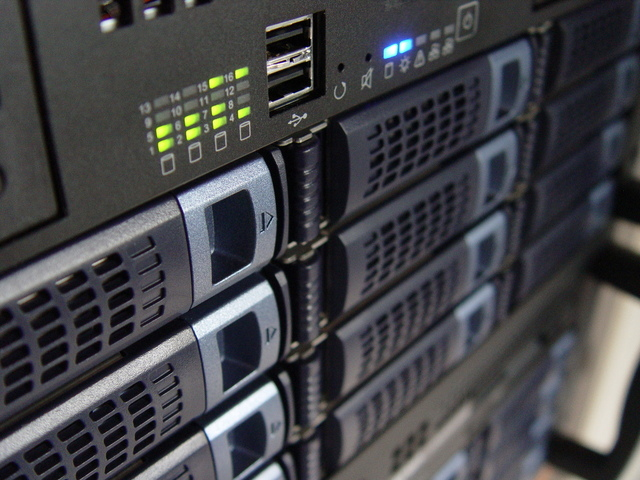
\includegraphics[scale=0.5]{servers.jpg}
}
\par\vspace{2cm}{
	Ultima fecha modificado: \today
}
\end{center}

% Indice
\clearpage
\section{Desarrollo}
Para esta practica solo fue necesario seguir los pasos que dejo escrito el profesor así como el escribir todo de forma natural para la ejecución de la aplicación, o en su defecto desarrollar un script que realice todas las tareas necesarias que permitan la automatización de la tarea a resolver, que es la instalación de todos los modulos (JDK 8, MySQL, Apache Tomcat, Webservice para REST)
\section{Códigos y scripts}
\subsection{Script para copia de datos a VM}
\lstinputlisting[language=Bash]{../script_cp.sh}
\subsection{Script para toda la automatización de crear la app web}
\lstinputlisting[language=Bash]{../script_rest.sh}
\subsection{Códigos de SQL que forman parte de script\_rest.sh}
\lstinputlisting[language=SQL]{../conf_root.sql}
\lstinputlisting[language=SQL]{../add_hugo.sql}
\lstinputlisting[language=SQL]{../web_rest.sql}
\subsection{Código de llenado de datos con Python}
\lstinputlisting[language=Python]{../script_fill.py}

Con esto finalmente solo es necesario abrir la aplicación web desde nuestro navegador, destacando que hay que dar un forwarding del puerto 8080
\section{Capturas}
\begin{center}
  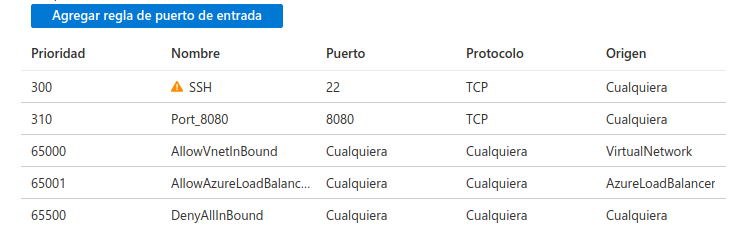
\includegraphics[scale=0.45]{imgs/config_ports.png}
  \\\textit{Figura 1: Pantalla de configuración de puertos de la VM}
  \begin{landscape}
    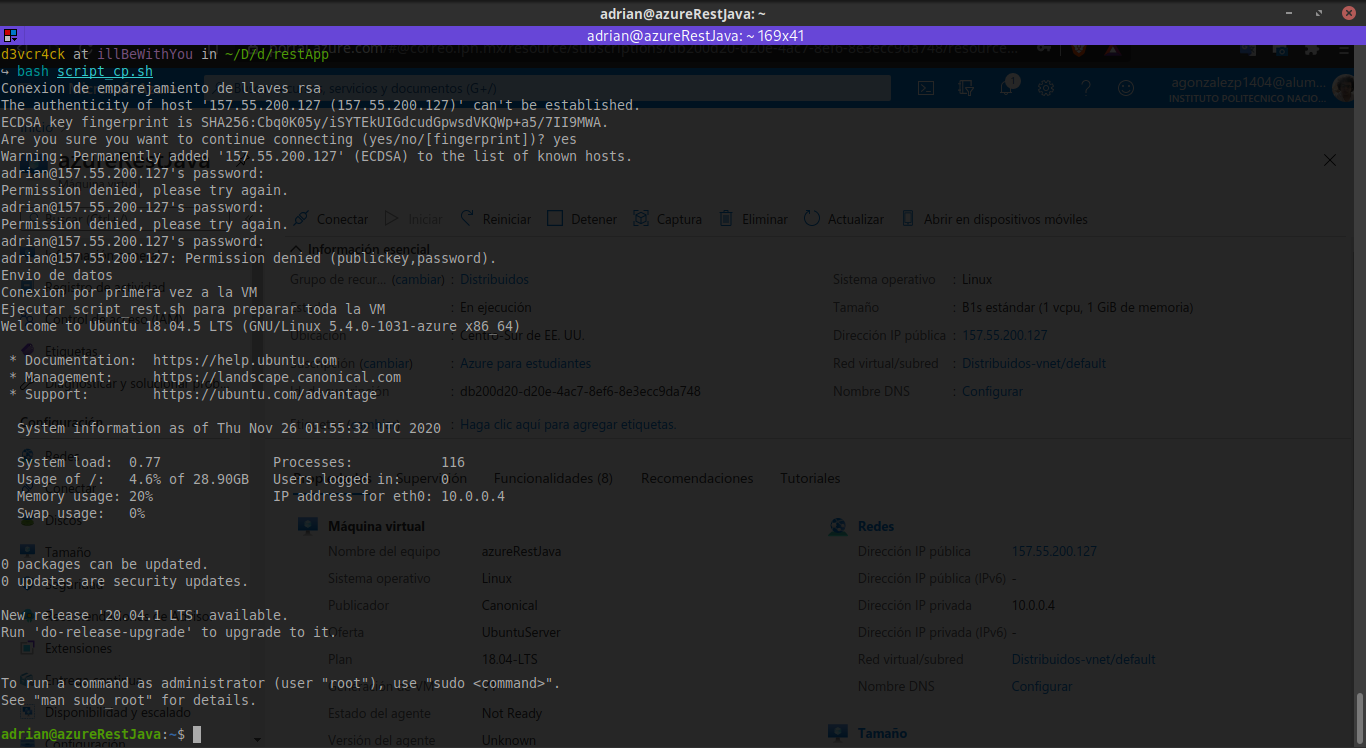
\includegraphics[scale=0.5]{imgs/conexion.png}
    \\\textit{Figura 2: Ejecución del primer script para conectarse con la VM}
    \fillandplacepagenumber
    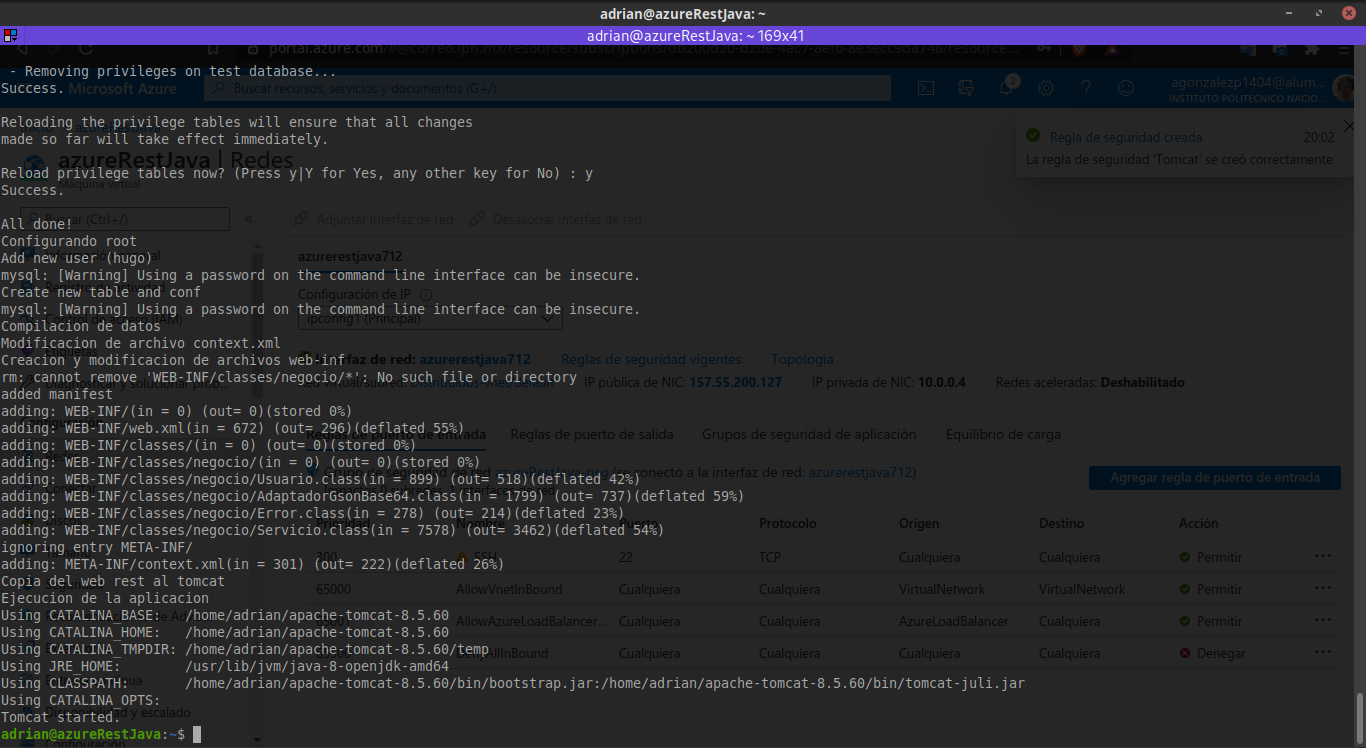
\includegraphics[scale=0.5]{imgs/script_install_rest.png}
    \\\textit{Figura 3: Ejecución del segundo script para instalar todo la aplicación REST}
    \fillandplacepagenumber
    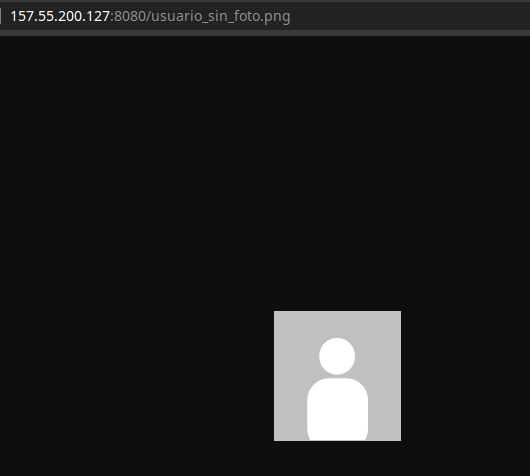
\includegraphics[scale=0.5]{imgs/rest_image.png}
    \\\textit{Figura 4: Primer parte de la aplicación REST}
    \fillandplacepagenumber

    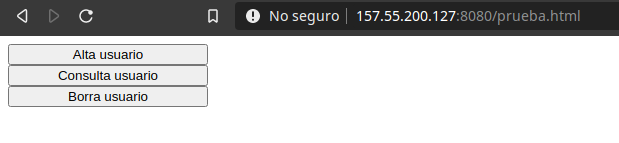
\includegraphics[scale=0.5]{imgs/html.png}
    \\\textit{Figura 5: Segunda parte de la aplicación REST vista de los botones}
    \fillandplacepagenumber

    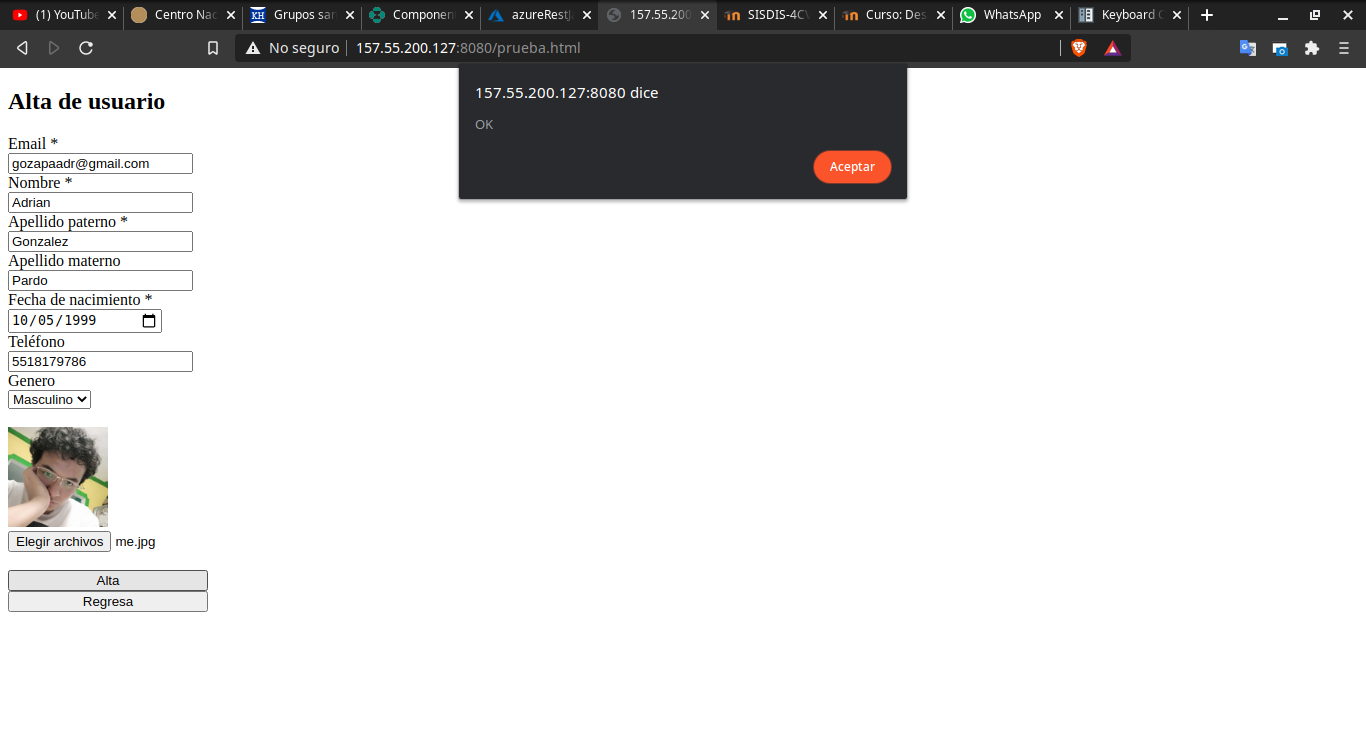
\includegraphics[scale=0.45]{imgs/ventana-captura.png}
    \\\textit{Figura 6: Segunda parte de la aplicación REST captura de datos de forma automatica}
    \fillandplacepagenumber

    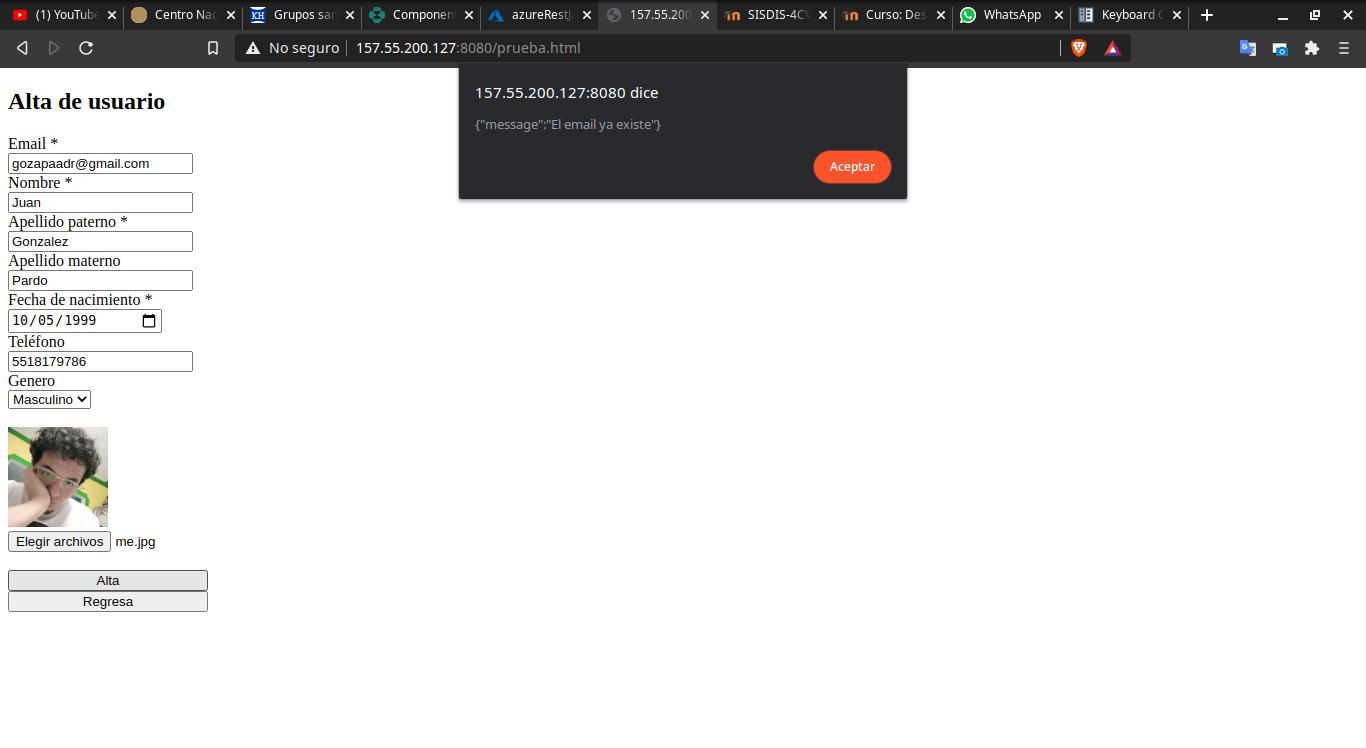
\includegraphics[scale=0.45]{imgs/otros-valores.png}
    \\\textit{Figura 7: Segunda parte de la aplicación REST captura de datos con redundancia en el correo (Cambia nombre)}
    \fillandplacepagenumber

    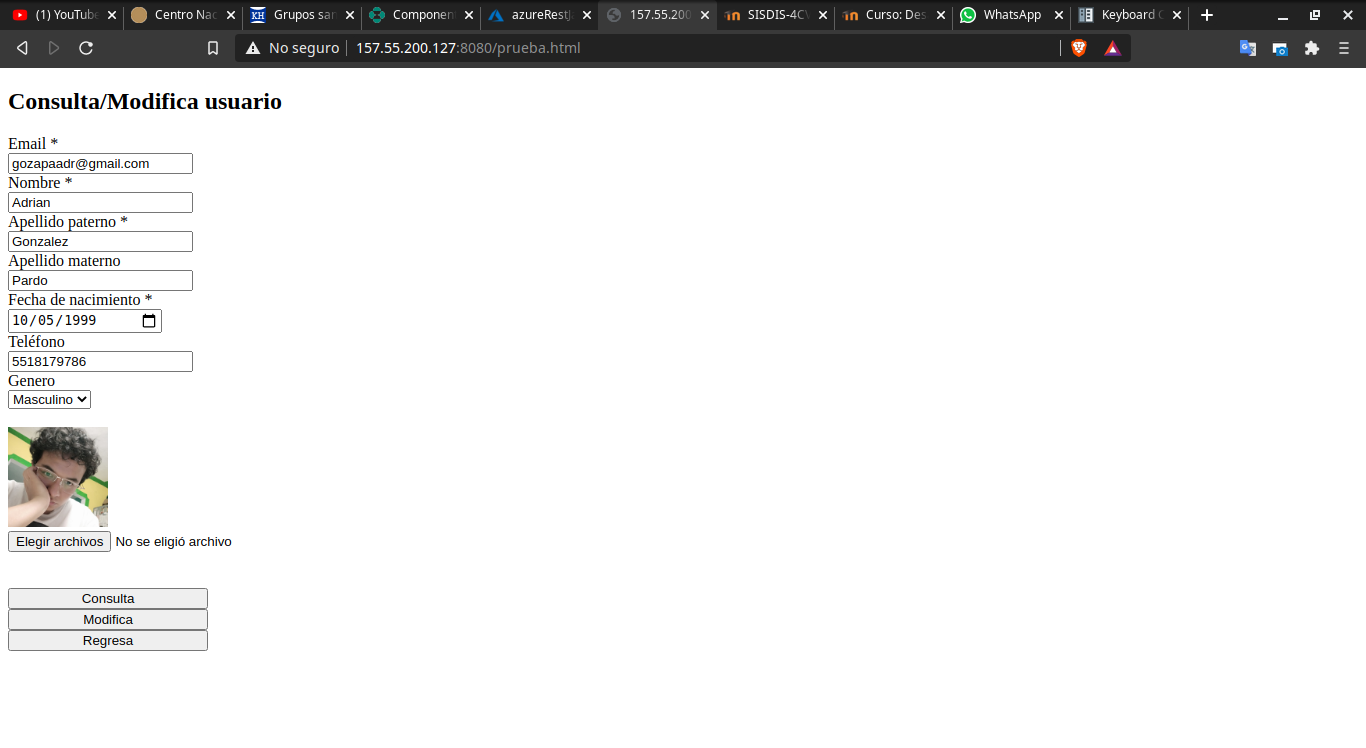
\includegraphics[scale=0.45]{imgs/consulta.png}
    \\\textit{Figura 8: Segunda parte de la aplicación REST consulta de datos}
    \fillandplacepagenumber

    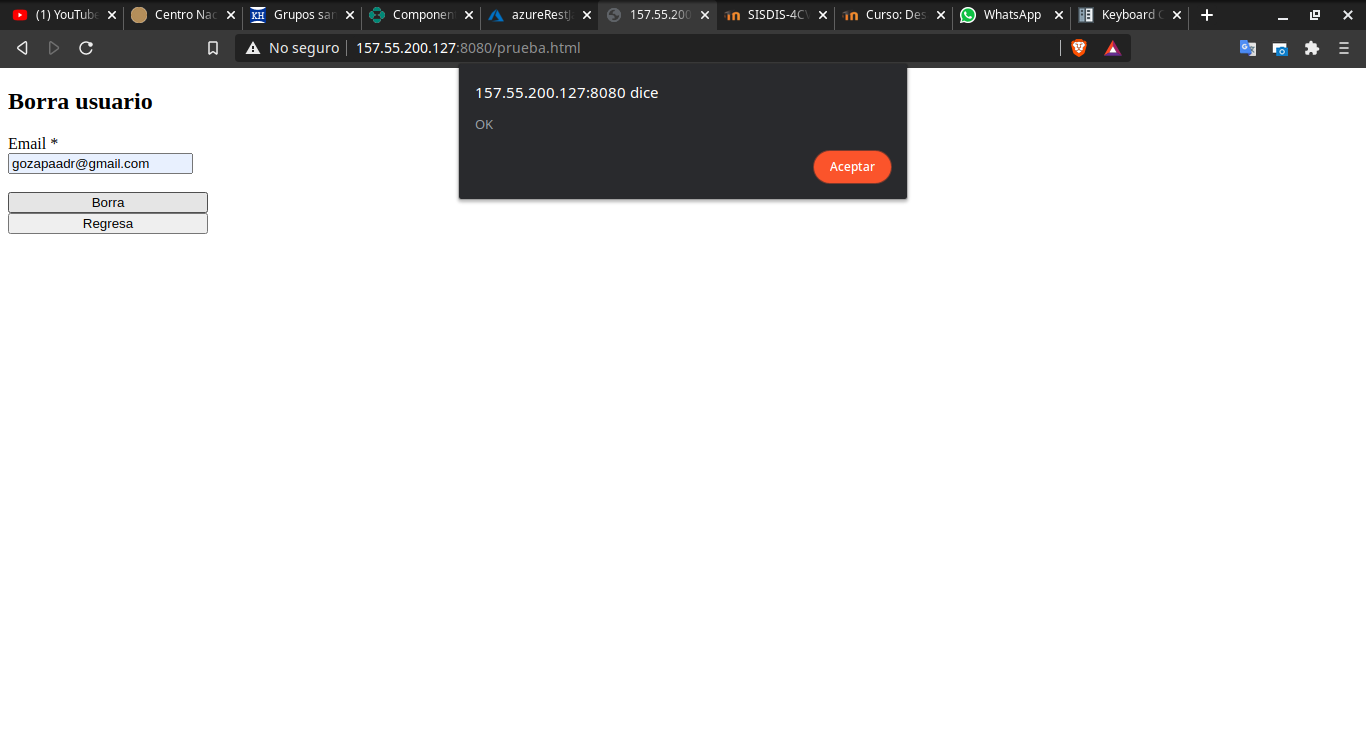
\includegraphics[scale=0.45]{imgs/eliminacion.png}
    \\\textit{Figura 9: Segunda parte de la aplicación REST eliminacion de datos}
    \fillandplacepagenumber

    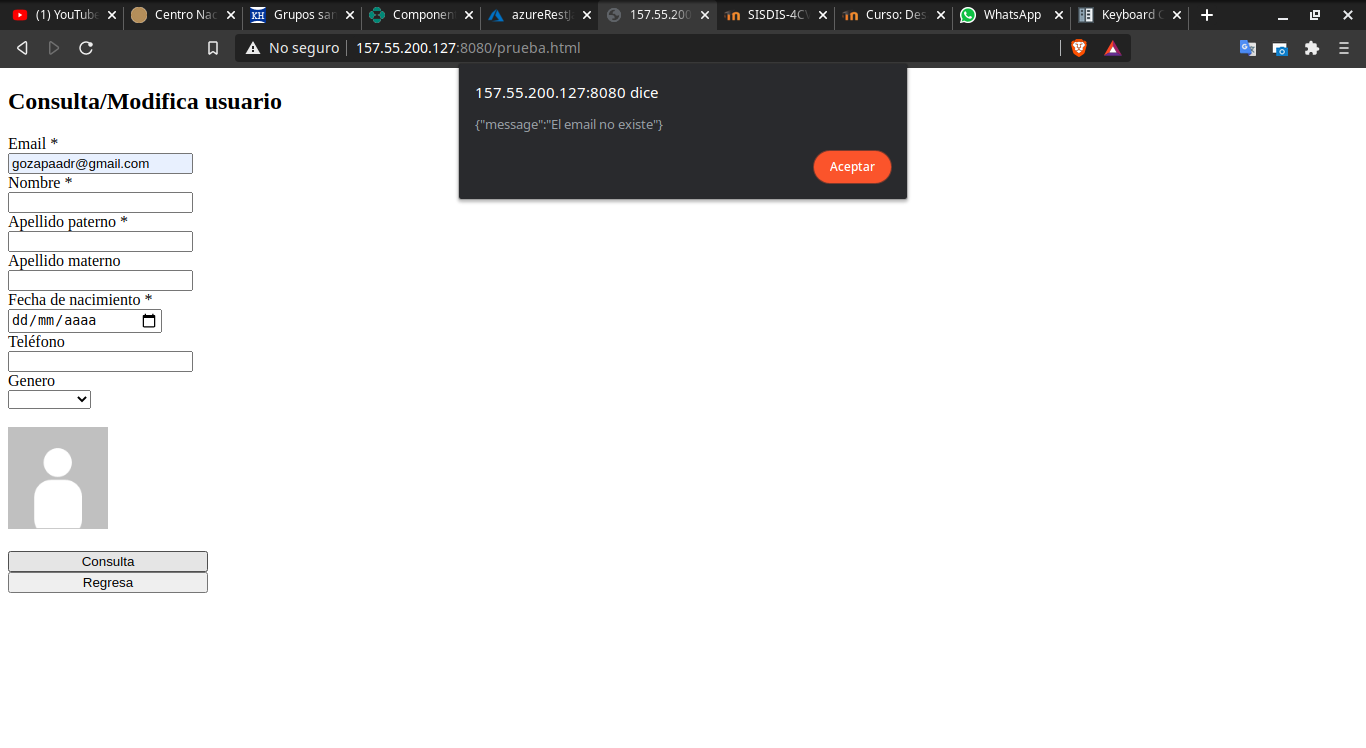
\includegraphics[scale=0.45]{imgs/consulta-des-eli.png}
    \\\textit{Figura 10: Segunda parte de la aplicación REST consulta de datos despues de eliminar}
    \fillandplacepagenumber
  \end{landscape}
\end{center}

\section{Conclusiones}
El realizar aplicaciones basadas en webservices como lo es REST nos permite saber el como trabajan algunas aplicaciones a la hora de almacenar y manejar ciertos, datos, si bien Java puede ser visto como una alternativa para esto, tambien existen otros lenguajes en conjunto de sus frameworks como lo son Ruby on Rails, Sinatra (Ruby), Django (Python), Flask (Python), Go, entre otros lenguajes más que nos permiten hacer aplicaciones REST es importante como se realizaban con lenguajes un poco más antaños como lo es Java.
\end{document}
